\chapter{W Bosons at the LHC}

\section{Introduction}

\PW boson production is an important process for physics studies at the LHC.  At
the \ac{LHC}, \PW bosons are produced at a high rate while offering a clean
experimental signal with a final state consisting of, in the case of a
leptonically decaying \PW, a single high \PT lepton with a large amount of
missing transverse energy due to the neutrino in the event. 

The production of \PW, through the \ac{DY} process, provides important
information on the interacting partons within the colliding hadrons.

\section{W Boson Production}

The dominant production process for a \PW boson at a hadron-hadron collider is
shown in \EquationRef{wbos:wprod}

\begin{equation}
  h_1(P_1) + h_2(P_2)
  \to 
  \PW + X
  \to
  \Pe \Pnue + X
  \label{wbos:wprod}
\end{equation}

\begin{figure}[htb]
  \centering
  %
\includegraphics[width=0.5\textwidth]{placeholder}
  \missingfigure{Make a diagram of W production. Not a feynman diagram.}
  \caption{Diagram of a W boson production at a hadron-hadron collider.}
  \label{wbos:wproddiag}
\end{figure}

This process is shown in \FigureRef{wbos:wproddiag}. 
The \PW boson is produced by the collision of the two incoming hadrons $h_1$
and $h_2$ with momenta $p_1$ and $p_2$. The \PW then decays leptonically to an
electron and its corresponding neutrino. $X$ represents the accompanying final
state.

At hadron colliders the full cross section is a convolution of the cross-section
at the parton level, and the \acp{PDF}.

\begin{multline}
  d\sigma_{(\HepProcess{h_1 h_2 \to \PWpm})}(p_1,p_2) = \\
  \sum\limits_{a,b}
  \int_0^1 \! \mathrm{d} x_1 
  \int_0^1 \! \mathrm{d} x_2 
  f_a^{h_1}(x_1,Q^2)
  f_b^{h_2}(x_2,Q^2) 
  d\hat{\sigma}_{(\HepProcess{a b \to \PWpm})}(x_1 p_1, x_2 p_2; Q^2)
  \label{wbos:xsec}
\end{multline}

where $\sum\limits_{a,b}$ represents the sum over the initial parton states $a$
and $b$, $f_a^{h}(x,Q^2)$ represents the \acp{PDF} and
$d\hat{\sigma}_{(\HepProcess{a b \to \PWpm})}(x_1 p_1, x_2 p_2; Q^2)$
represents the partonic sub-process cross-section.

\subsubsection*{Partonic Sub-Process}

At \ac{LO} the process for a \PWp is
\begin{equation}
  \HepProcess{\Pup + \APdown \to \PWp \to \Pleptonplus \Pnulepton} 
  \label{wbos:wpprod} 
\end{equation}
and for a \PWm:
\begin{equation}
  \HepProcess{\APup + \Pdown \to \PWm \to \Pleptonminus \APnulepton}
  \label{wbos:wmprod} 
\end{equation}

A tree-level Feynman diagram representing this process is shown in
\FigureRef{wbos:feynman}.

\begin{figure}[htb]
  \centering
  %
\includegraphics[width=0.5\textwidth]{placeholder}
  \missingfigure{Make a feynman diagram of W production, qqbar > W > l nu.}
  \caption{Tree-level diagram of a W boson production at a hadron-hadron collider.}
  \label{wbos:feynman}
\end{figure}

At the \ac{LHC} (a proton-proton collider), one parton is most to likely be a
valence quark with a high fraction of the protons momentum, and the other
parton will tend to be a sea anti-quark with a lower fraction of the momentum
than the quark. The difference in momentum of the partons causes the \PW bosons 
to tend to be produced at high rapidities. 

%It follows from \EquationRef{wbos:prod} that and difference in distributions of
%the $\Pup$ and $\Pdown$ quarks or the $\APup$ and $\APdown$ anti-quarks will
%cause the cross-section for \PWp and \PWm production to differ.

%A measurement of
%the distribution of the \PW bosons rapidities at the \ac{LHC} provides direct
%information on the quark and anti-quark densities of the proton at a high scale
%and low values of the parton momentum fraction. 

\subsubsection*{\acp{PDF}} 
The \ac{PDF} represents the number density of parton $a$ that has a momentum
fraction $x+\mathrm{d}x$ of the colliding hadron $h$.  \acp{PDF} are obtained
from global fits to experimental data.\cite{Martin:2009iq} %TODO more?

\begin{figure}[htb]
  \centering
  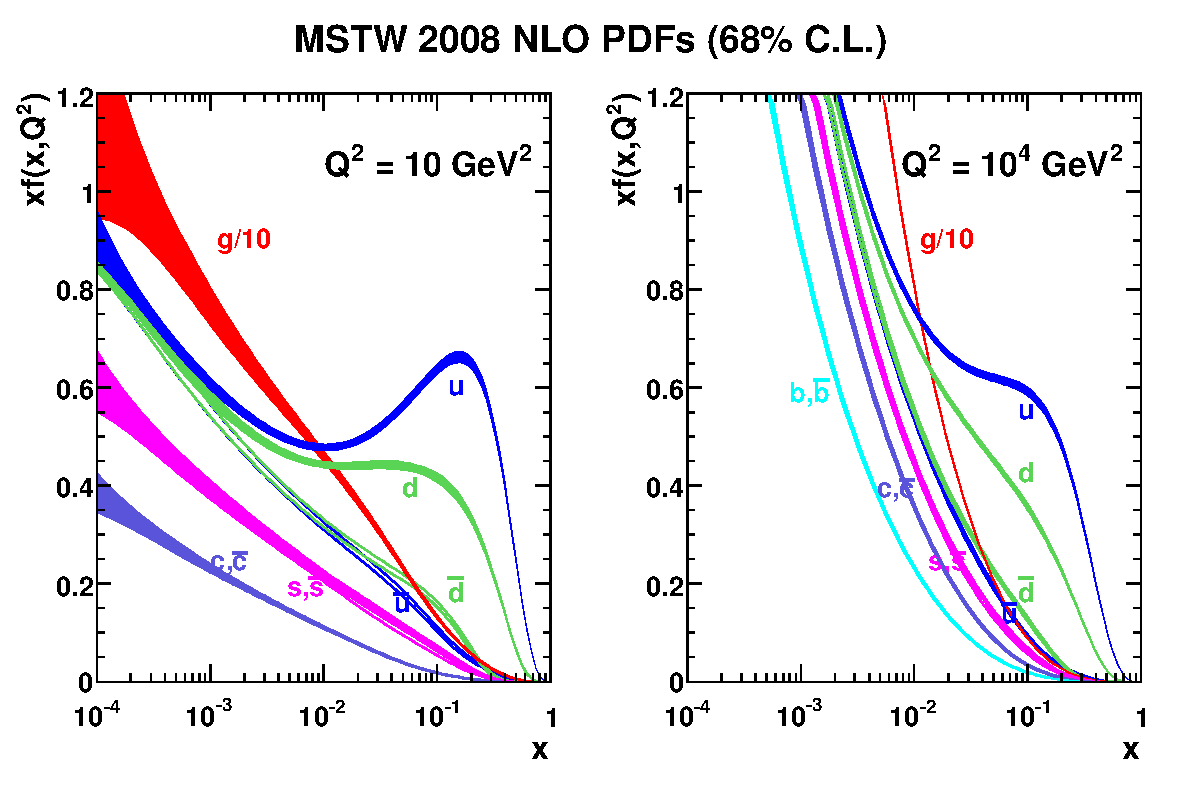
\includegraphics[width=\textwidth]{mstw2008nlo68cl_allpdfs}
  \caption{Proton PDF at  $ Q^2 = \unit{ 10  }{\GeV^2} $ (left) 
                      and $ Q^2 = \unit{ 100  }{\GeV^2} $ (right) 
                     from \cite{Martin:2009iq}. }
  \label{wbos:pdf}
\end{figure}

\FigureRef{wbos:pdf} shows the proton PDF at $Q^2\approx M_{\PW}^2$.  The
anti-quark parton densities $\APup(x,Q^2)$ and $\APdown(x,Q^2)$ are relatively
similar especially at the LHC energies, where the parton momentum fraction, x,
tends to be small.

The \ac{PDF} for the valence quarks in the proton differ, the up-type quark
dominates over the down-type. This is mainly due to the valence quark content
of the proton (\HepProcess{\Pup\Pup\Pdown}).  This can be seen in the
ratio of the up-type and the down-type \acp{PDF}, $R_{ud}(x,Q^2)$, given by:

\begin{equation}
  R_{ud}(x.Q^2) = \frac{\Pup(x,Q^2)}{ \Pdown(x,Q^2)} > 1
\end{equation}

Where $\Pup(x,Q^2)$ are the up and down quark \acp{PDF}.  
The ratio $R$ is a function of $x$, $R \approx 1$ for $x<<1$ and increases
monotonically as $x$ increases.  
% TODO why?

\section{\PW Boson Rapidity Distribution}
\label{wbos:wrapsec}

The rapidity distribution for \PWp and \PWm at the \ac{LHC} is shown in
\FigureRef{wbos:wrapid}. 
%TODO talk about how this plot was made
The \PWm distribution is shown in the left panel and the \PWp distribution is
shown in the right panel. The distributions are invariant with respect to the
flipping the rapidity, $y\leftrightarrow-y$, so are shown on a folded rapidity
axis.
%TODO make that make sense.

\begin{figure}[htb]
  \centering
  %
\includegraphics[width=0.5\textwidth]{placeholder}
  \missingfigure{Produce a plot of W rapidity at 7TeV proton-proton}
  \caption{The rapidity distribution for \PWp and \PWm at the LHC.}
  \label{wbos:wrapid}
\end{figure}

In \FigureRef{wbos:wrapid} the \PWp cross section is greater than the \PWm
cross section. This is a consequence of the different production processes for
\PWp (\EquationRef{wbos:wpprod}) and \PWm (\EquationRef{wbos:wmprod}) and the
\ac{PDF} for the valence quarks in the proton differing as seen in
\FigureRef{wbos:pdfrat}. The up-type quark \ac{PDF} dominates over the
down-type which leads to a greater \PWp production rate than \PWm.

It is also seen in \FigureRef{wbos:wrapid} that the \PWm tends to be produced
more centrally where as the \PWp is produced at larger rapidities. This is due
to \Pup quarks tending to carry a greater fraction of the protons momentum,
$x$, than the \Pdown type quarks as seen in \FigureRef{wbos:pdfrat}.

The momentum fraction, x, of the interaction quarks is correlated
with the rapidity of the \PW boson. The ratio of $\Pup$ and $\Pdown$ quarks as
a function of momentum fraction, $x$, is directly related to the difference in
cross-sections for \PWp and \PWm production as a function of the boson
rapidity.

Therefore a measurement of the asymmetric production of \PW bosons, as a
function of the rapidity of the boson, at the \ac{LHC} provides important
information on the ratio of the up-type and down-type quark parton densities as
a function of x,
$R_{ud}(x,Q^2)$, within the proton. 

\section{\PW Boson Charge Asymmetry}

% formalised def of w asymmetry
The \PWpm boson charge asymmetry is defined as:

\begin{equation}
  A_{W}(y_{\PW})=
    \frac{ 
      \nicefrac{ d\sigma (\PWp) }{ dy_{W} } -
      \nicefrac{ d\sigma (\PWm) }{ dy_{W} }
    }
    {
      \nicefrac{ d\sigma (\PWp) }{ dy_{W} } +
      \nicefrac{ d\sigma (\PWm) }{ dy_{W} }
    }
\label{wbos:wasym}
\end{equation} 

Where $y_{W}$ is the boson rapidity, and 
$\nicefrac{ d\sigma (\PWpm) }{ dy_{W} }$ is the \PWpm production cross section
at a fixed $y_{W}$.  
If $d\sigma(\PWp) > d\sigma(\PWm) $ then $A_{W}(y_{\PW})> 0$,
else if $d\sigma(\PWp) < d\sigma(\PWm) $ then $A_{W}(y_{\PW})< 0$,
and for symmetric \PWpm boson production, $A_{W}(y_{\PW})= 0$,

The prediction for the W boson charge asymmetry as a function of the boson
rapidity is shown in \FigureRef{wbos:chargeasym}. $A_{W}(y_{\PW})> 0$ and
increases as the rapidity increases.

\begin{figure}[htb]
  \centering
  %
\includegraphics[width=0.5\textwidth]{placeholder}
  \missingfigure{Produce a plot of W asymmetry at 7TeV proton-proton}
  \caption{\PW boson charge asymmetry at LHC.}
  \label{wbos:chargeasym}
\end{figure}

\PW bosons are identified by their decay to a lepton plus neutrino, however at
hadronic colliders the neutrino longitudinal momentum can not be determined
which means that the \PW rapidity, $y_{W}$, can not be measured.  Instead what
is studied is the lepton charge asymmetry.

%It is possible to overcome the difficulty in determining the boson rapidity
%by extrapolating the neutrino longditudinal momentum from the lepton neutrino
%with a \ac{MC} study. 

\section{Electron Rapidity Distribution}

The rapidity distributions of the charged lepton produced from \PW decay are
further complicated by the charge asymmetric decay of the \PWpm boson. 
The asymmetric decay arises due to the $V-A$ coupling of the \PW boson to the
annihilating \HepProcess{\Pquark\APquark} pair and the decaying lepton pair.

At \ac{LO} the \PWp is produced in the annihilation of a \Pup valance quark
with a \APdown sea-quark (\EquationRef{wbos:wpprod}). 
If the parton masses are neglected the \Pup is left-handed and the \APdown is
right-handed, as shown at the top of \FigureRef{wbos:wspin}. 

In the \PWp decay the \Ppositron is right-handed and the \Pnue is left-handed.
\FigureRef{wbos:wspin} shows if the  positron is produced in the same direction
as the incoming \APdown quark angular momentum is conserved and the decay is
allowed.
However the decay where the positron is produced in the same direction as the
incoming \Pup quark, is forbidden.
A similar argument holds true for \PWm decays, where the \Pelectron is produced
preferentially in the direction of the \Pdown.

\begin{figure}[htb]
  \centering
  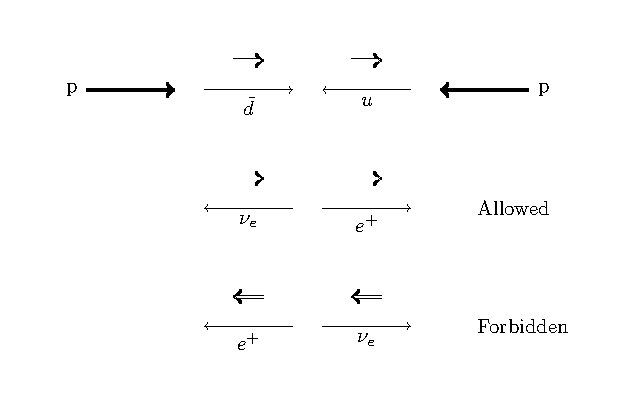
\includegraphics[width=0.8\textwidth]{w_decay_directions}
  \caption{Preferred directions of electrons in \Wenu decay.\cite{TODO}}
  \label{wbos:wspin}
\end{figure}

The actual distribution of the electron from \PWpm decay is given by\cite{}

\begin{equation}
  \frac{1}{\sigma_{U\bar{D}}}
  \frac{d \sigma_{U\bar{D}}}{d \cos \theta_{\Plepton D}^{\ast}}
  =
  \frac{1}{\sigma_{D\bar{U}}}
  \frac{d \sigma_{D\bar{U}}}{d \cos \theta_{\Plepton D}^{\ast}}
  =
  \frac{3}{8}(1+\cos \theta_{\Plepton D}^{\ast})^2
  \label{wbos:lepton}
\end{equation}

where $\theta_{\Plepton D}^{\ast}$ is the scattering angle of the charged
lepton with respect to the direction of the down-type quark or anti-quark, in
the centre of mass system of the two quarks. The cross-section is maximised when
$\theta_{\Plepton D}^{\ast}$ is minimised and the charged lepton is produced in
the same direction as the down-type quark.

The rapidity distribution of the electron is therefore a convolution of the
\ac{EWK} correlations in \EquationRef{wbos:lepton} with the \PW rapidity
described in \SectionRef{wbos:wrapsec}:

\begin{equation}
  y_{\Plepton} = 
  y_{\PW} +
  \frac{1}{2}
  \ln
  \frac{1 + \cos \theta_{\Plepton D}^{\ast}}{1 - \cos \theta_{\Plepton D}^{\ast}}
  \label{wbos:leptonfull}
\end{equation}

In proton-proton collisions the \PWp tends to be produced in the direction
of the \Pup, as described in the preceding chapter.  
However, due to the EWK correlations the charged lepton from the decaying \PWp
will tend to be produced along the direction of the down type quark and
therefore will shift the rapidity distribution of the lepton to be more
centrally.\cite{}

Similarly, \PWm bosons tend to be produced more centrally, however the EWK
correlations will shift the charge lepton rapidity distribution to higher rapidities.

\begin{figure}[htb]
  \centering
  %
\includegraphics[width=0.5\textwidth]{placeholder}
  \missingfigure{Produce a plot of lepton asymmetry at 7TeV proton-proton}
  \caption{Electron and positron rapidity distributions.}
  \label{wbos:leptonrapidity}
\end{figure}

\section{Electron Charge Asymmetry}

The electron asymmetry is defined in \EquationRef{eq:AsymThe} analogously to the
\PW boson asymmetry in \EquationRef{wbos:wasym}, as the difference in the
\inclusiveWe cross-section over the total \inclusiveWe cross-section.

\begin{equation}
A_{the}(\eta)=\frac{  \frac{d\sigma}{d\eta}(\Wpenu) -
\frac{d\sigma}{d\eta}(\Wmenu) }{ \frac{d\sigma}{d\eta}(\Wpenu) +
\frac{d\sigma}{d\eta}(\Wmenu) }
\label{eq:AsymThe}
\end{equation} 

In an experiment, the cross-section is not measured directly, instead what is
measured is the electron and positron yields.  The experimentally measured
asymmetry is given by equation \ref{eq:AsymExp}.\cite{kom}
 
\begin{equation}
A_{exp}(\eta)=\frac{  \frac{dN}{d\eta}(\Pelectron) -
\frac{dN}{d\eta}(\APelectron) }{ \frac{dN}{d\eta}(\Pelectron) +
\frac{dN}{d\eta}(\APelectron) }
\label{eq:AsymExp}
\end{equation} 

To get from the experimentally measured asymmetry to the lepton charge
asymmetry, \EquationRef{eq:NumEve} must be used, which takes in to
account the experimental effects such as the luminosity (${\cal L}$), high
level trigger ($\epsilon_{HLT}$), offline efficiency ($ \epsilon_{off}$) and
the acceptance ($\epsilon_{acc}$).

\begin{equation}
\frac{dN}{d\eta} = {\cal L } \frac{d\sigma}{d\eta}  \epsilon_{HLT}
\epsilon_{off} \epsilon_{acc}
\label{eq:NumEve}
\end{equation} 

Since the asymmetry is a ratio, the luminosity, high level trigger and the
offline efficiency can be cancelled out assuming that they are not asymmetric
with respect to charge.\cite{me} 

The acceptance can not be cancelled however, since it is a function of rapidity and 
these distributions will differ for \Pelectron and \APelectron.
The experimentally measured asymmetry can therefore be related to the
theoretical asymmetry by correcting for the acceptance.\cite{me}

\begin{align} 
A_{exp}(\eta) &= \frac{ \frac{dN}{d\eta}(\Pelectron) -
\frac{dN}{d\eta}(\APelectron) }{ \frac{dN}{d\eta}(\Pelectron) +
\frac{dN}{d\eta}(\APelectron) }\\   
              &= \frac{ \frac{d\sigma}{d\eta}(\Wpenu) -
\frac{\epsilon^{-}_{acc}}{\epsilon^{+}_{acc}} \frac{d\sigma}{d\eta}(\Wmenu) }{
\frac{d\sigma}{d\eta}(\Wpenu) + \frac{\epsilon^{-}_{acc}}{\epsilon^{+}_{acc}}
\frac{d\sigma}{d\eta}(\Wmenu) }
\label{eq:AsymExpCorr}
\end{align}

\section{Electron Charge Asymmetry Theoretical Predictions}

In this section the electron charge asymmetry predictions are studied in detail.
Predictions for the asymmetry are obtained using MCFM \cite{test} generator
interfaced with MSTW2008NLO PDF models unless otherwise stated.

\FigureRef{wbos:asym_simple} shows the electron charge asymmetry prediction for
electron transverse momentum cuts of 25, 30 and \unit{35}{\GeV}.


\begin{figure}[htb]
  \centering
  %
\includegraphics[width=0.5\textwidth]{placeholder}
  \missingfigure{Produce a plot of lepton charge asymmetry at 7TeV proton-proton
cut of 25,30 and 35 GeV.}
  \caption{Electron charge asymmetry (simple).}
  \label{wbos:asym_simple}
\end{figure}
% simple prediction to illustrate the preceeding chapter on electron charge
% asymmetry

Unlike the \PW asymmetry , the electron asymmetry turns over at $\eta\approx
2.5$ due to the effect of the the \ac{EWK} correlations.

\subsection{Uncertainty on \acp{PDF}}

The predictions of the electron charge asymmetry will have an error associated
with the uncertainty on the \ac{PDF}.
The uncertainty on the \ac{PDF} originates from the experimental errors on the
data used in the global fits.

The \ac{PDF} uncertainty is propagated to the electron charge asymmetry
measurement using the \ac{PDF} re-weighting techniques\cite{}.
%TODO add more here

\begin{figure}[htb]
  \centering
  %
\includegraphics[width=0.5\textwidth]{placeholder}
  \missingfigure{Produce a plot of lepton charge asymmetry at 7TeV proton-proton
cut of 25 GeV with PDF uncertainties.}
  \caption{Electron charge asymmetry (PDF uncertainty).}
  \label{wbos:asym_pdfuncert}
\end{figure}

\FigureRef{wbos:asym_pdfuncert} shows the prediction for the electron charge
asymmetry with a \PT cut of \unit{25}{\GeV} with the \ac{PDF} uncertainty shown.

%TODO EVAL RESULTS

% uncertainty on PDF
% FIXME might not include this part

%\subsection{Theoretical Uncertainty Due To Higher Orders}
%\begin{figure}[htb]
%  \centering
%  
\includegraphics[width=0.5\textwidth]{placeholder}
%  \caption{Electron charge asymmetry (LO, NLO and NNLO).}
%  \label{wbos:asym_NNLO}
%\end{figure}
% difference in NLO and NNLO give an estimate on the uncertainty on the
% partonic subprocess

\subsection{Choice of \acp{PDF}}

The predictions of the electron charge asymmetry will depends on the choice of
\ac{PDF} used. 
\FigureRef{wbos:asym_pdf} shows the electron charge asymmetry for
various \ac{PDF} models.

\begin{figure}[htb]
  \centering
  %
\includegraphics[width=0.5\textwidth]{placeholder}
  \missingfigure{Produce a plot of lepton charge asymmetry at 7TeV proton-proton
cut of 25 GeV with different PDFs.}
  \caption{Electron charge asymmetry (Many PDF sets central values...?).}
  \label{wbos:asym_pdf}
\end{figure}

% statment about disagreement and how this measurement will help

%\begin{figure}[htb]
  %\centering
  %
\includegraphics[width=0.5\textwidth]{placeholder}
  %\caption{Electron charge asymmetry (Many PDF sets ratio to MSTW with PDF
  %uncert).}
  %\label{wbos:asym_ratio}
%\end{figure}






